\section{Segment Anything Model} \label{sec:sam}

The Segment Anything Model (SAM) \cite{kirillov2023segany} is a state-of-the-art tool for image segmentation. It is designed as a general-purpose segmentation model that works across a wide range of images. However, the samples used in this work are very specific, and pixel-level precision is crucial.

As shown in Figure~\ref{fig:sam_subfigures}, even when using five positive and nine negative points to guide the segmentation, SAM struggles to distinguish between the coating and the upper oxidation layer. This is not ideal, as researchers would need to manually place many guidance points for each measurement and still often need to refine the mask using a brush tool.

Another key limitation of SAM is its high hardware requirements. Running it on a standard office computer, essential for automating the measurement process, is not feasible. Unlike smaller models that can operate locally, SAM demands either a dedicated GPU or a remote server setup, neither of which is a viable option in this case.

Additionally, SAM requires user input through interactive prompts, creating a significant technical hurdle, particularly since the model needs to be integrated into Fiji. Adapting it within Fiji would require considerable adjustments to external software, introducing unnecessary complexity to the workflow.

\begin{figure}[H]
    \centering
    \begin{subfigure}[b]{0.7\linewidth}
        \centering
        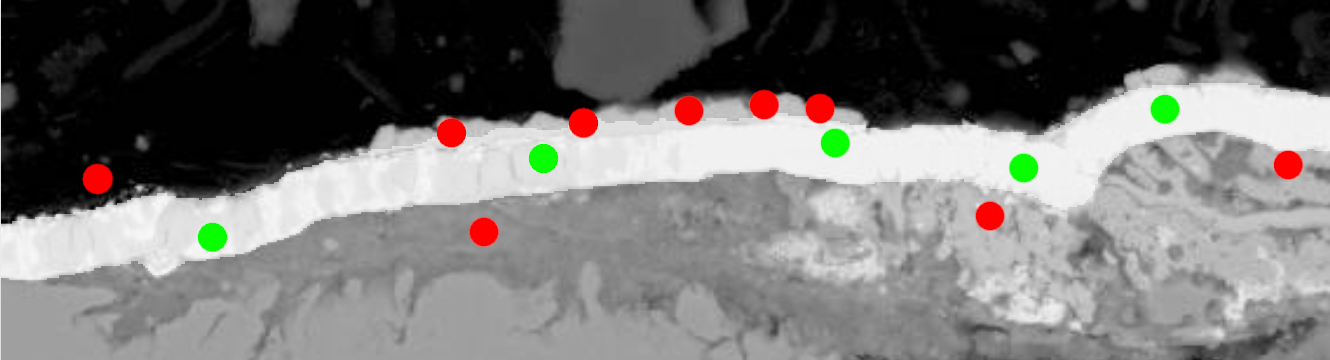
\includegraphics[width=\linewidth]{PICTURES/SAM/points_sam_small.png}
        \caption{User-provided positive (green) and negative (red) points used to guide the SAM segmentation.}
        \label{fig:input_points}
    \end{subfigure}
    \vspace{0.5cm} % Adjust space between the subfigures
    \begin{subfigure}[b]{0.7\linewidth}
        \centering
        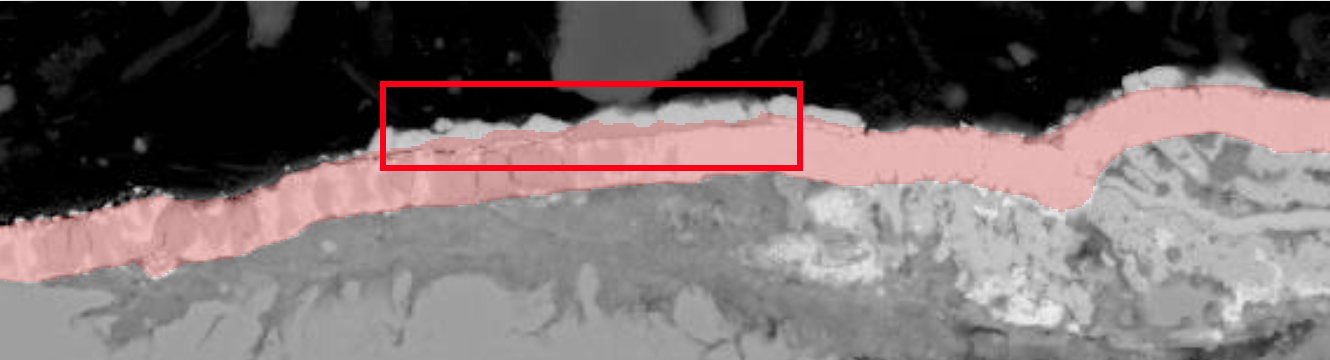
\includegraphics[width=\linewidth]{PICTURES/SAM/rect_small.png}
        \caption{Output mask generated by SAM. The red rectangle highlights the difficulty distinguishing between the oxidation and coating layers.}
        \label{fig:output_mask}
    \end{subfigure}
    \caption{Top: User-provided points (input). Bottom: SAM-generated output mask.}
    \label{fig:sam_subfigures}
\end{figure}
